\chapter{Theory}

\section{Electron Microscopy}
In an electron microscope, a beam of electrons are transmitted onto a material. Compared to a microscope using visible light, an EM gives a much higher resolution due to the wavelength of electrons being much smaller than that of visible light. Because of this, an EM can be used to study the atomic structure of materials.

	\subsection{Electron-sample interaction}
When the electron beam hits the sample, several different signals are generated. This report will only discuss two of them: Characteristic X-rays (due to inelastically scattered electrons, and elastically scattered electrons. Characteristic X-rays are produced as the incoming electrons interact with inner-core electrons in the sample, and can be used to determine which elements the sample consists of. The theory behind characteristic X-rays, and why they are useful, will be expanded upon in section \ref{EDS}. Electrons being transmitted through the sample that are elastically scattered (that is, the energy of the incoming electrons is conserved) gives rise to a diffraction pattern, which can be used to determine the crystallographic properties of the sample. Electron diffraction will be properly introduced in section \ref{ED} \cite{williams-carter}.

	\subsection{Transmission Electron Microscopy (TEM)}
There are many different kinds of transmission electron microscopes (TEMs), of which only the scanning TEM (STEM), introduced in section \ref{STEM}, will be expanded upon here. Before discussing the STEM, however, the basics behind the TEM will now be presented. In a conventional TEM, a broad, parallel beam of electrons is transmitted through a sample. In order for a sufficient amount of electrons to be transmitted, the sample is required to be thin (a thickness of <$\SI{100}{\nano\meter}$ is common). A TEM typically operates with electron energies of $\SI{200}{\kilo\electronvolt}$ or $\SI{300}{\kilo\electronvolt}$, giving the electrons a velocity $v > c/2$ which requires relativistic effects to be taken into account. Another factor that should be considered is the possibility of the electron beam damaging the material. This can happen as the chemical bonds in the material are broken (radiolysis), atoms are displaced or ejected from the crystal lattice (knock-on damage or sputtering, respectively) or as the material is changed due to heating. \cite{williams-carter}

%	\subsection{Scanning Electron Microscopy (SEM)}

	\subsection{Scanning Transmission Electron Microscopy (STEM)}
A scanning transmission electron microscope (STEM) uses an electron beam focused onto a small spot on the sample. The sample is then scanned in a raster pattern and the signal is recorded for each point. This technique can be used to investigate very small areas of the sample and accurately study transitions in atomic structure and/or composition.

\section{X-ray spectroscopy}\label{EDS}
The characteristic X-rays resulting from inelastic scattering of the electrons being transmitted through the sample can be used for both qualitative and quantitative analysis. Qualitative analysis can determine which elements are in the sample, while quantitative analysis can indicate the composition of the different elements. When X-ray spectroscopy is performed in a STEM, the electron probe is scanned over the material and focused on each pixel for a certain amount of time. During this time period, the X-rays being emitted from the sample are detected and the signal for the pixel is saved before the probe moves to the next pixel. 

	\subsection{Energy-Dispersive X-Ray Spectroscopy (EDS)} % Taken in STEM!!
		\subsubsection{X-ray emission}
As previously mentioned, characteristic X-rays are produced due to inelastic scattering of the incoming electrons on the sample. If an electron reaches the inner-shell electrons of an atom in the sample, and a sufficient amount of energy is transferred to the inner-shell electron, the electron will be ejected from the nucleus. That is, it reaches an energy above the Fermi level and is no longer bound to the nucleus [CHECK THIS]. The atom is now in an excited state, and will seek to return towards its ground state. This leads to an electron in an outer shell taking the place of the ejected electron in the inner shell, and in the process emitting an X-ray or an Auger electron (Auger electrons will not be discussed further). If an X-ray is emitted, its energy will be characteristic of the specific element, as different elements have different critical ionization energies. The critical ionization energy is the energy required for an inner-shell electron to be ejected from the nucleus.

There will not necessarily only be emitted one characteristic X-ray for each hole created in the inner shell of an atom. This is because the outer-shell electron filling the hole will create a new hole in its shell, which must be filled by an electron in a shell even further out, and maybe emitting another characteristic X-ray. This process continues until there is a hole in the outermost shell of the atom that can be filled by an electron in the conduction or valence band of the material. The energy of the characteristic X-rays will also depend on which transition it is emitted because of. In addition, due to quantum effects the electron shells might be split into several sub-shells, further increasing the number of different energies the emitted X-rays can have.

The probability for a specific transition to occur must also be taken into account. If a transition between two specific shells has a relatively high probability compared to other transitions in the element, more characteristic X-rays with the corresponding energy will be emitted over a certain time period. This will lead to higher peaks in the EDS spectrum, which will be discussed shortly.

		\subsubsection{X-ray detection}
When doing EDS in a TEM, an X-ray detector is positioned above the sample to detect the X-rays emitted from it. The detector then measures the energy of each incoming X-ray, with a given energy resolution. If the measurement is done using STEM, the electron probe is scanned over the sample and kept at each pixel for a certain amount of time during which emitted X-rays are detected. When the scanning is complete, this results in a three dimensional EDS spectrum.

		\subsubsection{EDS spectrum}\label{sec:eds-spec}
In an EDS spectrum, the intensity of the X-rays is plotted against the energy of the X-rays. The intensity at a certain energy refers to the number of counts, that is, how many X-rays with that energy that were detected by the detector. An example of an EDS spectrum is shown in Figure \ref{fig:eds-example-spectrum}. By consulting a table of known X-ray energies for the emission lines from different elements, for example \cite{x-ray-booklet}, one can determine which elements are present in the sample. However, knowing which elements are present is not enough to determine the structure of the material. A next step can be to perform quantitative analysis on the same spectrum.

\begin{figure}
\centering
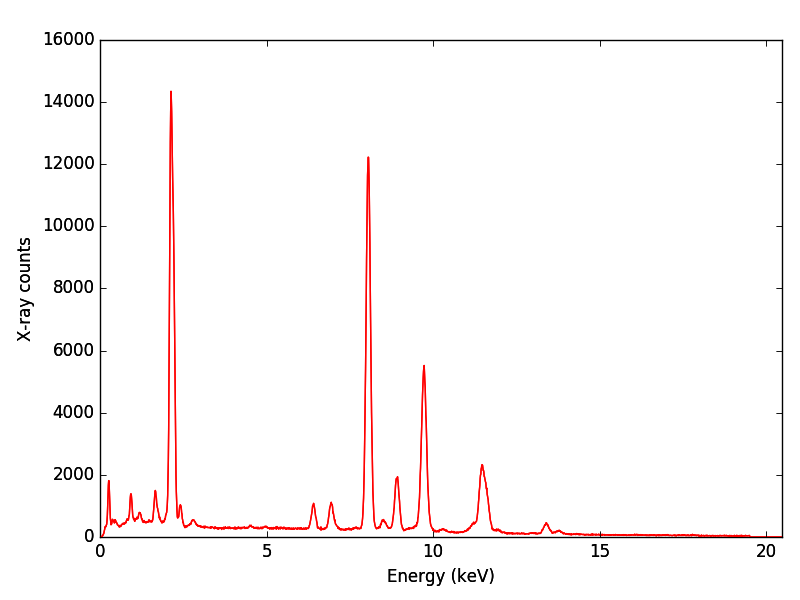
\includegraphics[width=0.7\linewidth]{fig/edx-example-spectrum}
\caption{Example of EDS spectrum}
\label{fig:eds-example-spectrum}
\end{figure}

	\subsection{Quantitative X-ray Analysis}
Quantitative analysis of an EDS spectrum gives information about the composition of the different elements in the material. A quantitative analysis might result in learning that an unknown material is a compound of a few different elements. In order to determine which compound this is, quantitative analysis is necessary.

There are primarily two methods for quantitative X-ray analysis: The Cliff-Lorimer ratio technique and the $\zeta$-factor method. The basis for both is assuming that the concentration of an element in a material is proportional to the intensity of characteristic X-rays being emitted from it, $C \propto I$.

		\subsubsection{The Cliff-Lorimer ratio technique}
The Cliff-Lorimer ratio technique, first introduced in 1972 \cite{cliff-lorimer}, assumes that the weight percent ratio of two elements is proportional to their intensity ratio,
\begin{equation}
\label{eq:CL-eq}
\frac{C_A}{C_B} = k_{AB}\frac{I_A}{I_B},
\end{equation}

where $C$ is the weight percent, $I$ is the intensity of the characteristic X-rays and the proportionality factor $k_{AB}$ is called the Cliff-Lorimer factor, or the $k$-factor. The $k$-factor depends not only on the properties of the elements $A$ and $B$, but also on the instruments used, the conditions under which the experiment was done, and how the intensities are extracted from the spectrum. This technique has several drawbacks: Firstly, determining the $k$-factor experimentally is very time-consuming, but a theoretical calculation can have a severe error \cite{williams-carter}. And secondly, the multi-element thin standards necessary for experimental determination are difficult to prepare.

		\subsubsection{The $\zeta$-factor method}
The $\zeta$-factor method was introduced by M. Watanabe and D. B. Williams in 1996, and overcomes several of the problems with the Cliff-Lorimer technique. If the material is a thin-film, its mass-thickness can be assumed to be proportional to the intensity of the characteristic X-rays $I$ and the composition $C$,

\begin{equation}
\label{eq:zeta-eq}
\rho t = \zeta \frac{I}{C D_e},
\end{equation}

where $\rho$ is the density of the material, $t$ is its thickness and $D_e$ is the total amount of electrons that hit the material during the measurement. 

Using the thin-film approximation to find a theoretical expression for the intensity $I$, the proportionality factor $\zeta$ can be found to be

\begin{equation}
\label{eq:zeta= }
\zeta = \dfrac{M}{N_v Q \omega a [\Omega/(4\pi)]\epsilon}.
\end{equation}

Here, $M$ is the atomic weight, $N_v$ is Avogadro's number, $Q$ is the ionization cross section, $\omega$ is the fluorescence yield, a is the relative transition probability, $\Omega/(4\pi)$ is the detector collection-angle and $\epsilon$ is the detector efficiency \cite{zeta-method}. If the composition and thickness of a material is known, equation \eqref{zeta-eq} can be used to calculate the $\zeta$-factor for the material.

Another advantage of the $\zeta$-factor method is the inclusion of absorption correction. The absorption correction-term for a specific X-ray line is given as

\begin{equation}
A = \frac{(\nicefrac{\mu}{\rho})_{sp}\rho t \mathrm{cosec} \alpha}{1-\exp[-(\nicefrac{\mu}{\rho})_{sp}\rho t \mathrm{cosec} \alpha]},
\label{eq:Abs-corr}
\end{equation}

where $(\nicefrac{\mu}{\rho})$ is the mass absorption coefficient of the characteristic X-ray line, and $\alpha$ is the X-ray take-off angle (++++++++ this is kinda plagiarizing). Absorption correction is implemented by multiplying this term to the intensity $I$ in \cref{eq:zeta-eq}, giving 
\begin{equation}
\rho t = \zeta \frac{I}{C D_e} A
\end{equation}

In a multi-element system, assuming the compositions obey $\sum_{j} C_j = 1$, \cref{eq:zeta-eq} gives the mass-thickness and composition of each element as
\begin{equation}
\rho t = \sum_j \frac{\zeta_j I_j A_j}{D_e}, \quad C_i = \frac{\zeta_i I_i A_i}{\sum_j \zeta_j I_j A_j}
\end{equation}

These equations can be solved through an iterative process: First, the mass-thickness and compositions are determined without absorption correction. Then the correction terms are calculated, and the mass-thickness and compositions are calculated with absorption correction. These last two steps are repeated until convergence is reached \cite{zeta-method}.

As both the $\zeta$-factor and the $k$-factor in \cref{eq:zeta-eq, eq:CL-eq} are proportional to the X-ray intensity and composition, the ratios for two elements should be roughly equal,

\begin{equation}
\label{compare_zeta_CL}
\frac{\zeta_A}{\zeta_B} \equiv \frac{k_{AB}} = \frac{k_{AX}}{k_{BX}},
\end{equation}

where $X$ denotes the element which the $k$-values have been measured with respect to (usually Si).

\section{Electron diffraction}\label{ED}
When electron diffraction is performed in a TEM, a beam of electrons is transmitted through the specimen. As the electrons pass through, some are scattered due to the atomic potentials in the specimen. By detecting the positions of the electrons after they have been transmitted through the specimen, a diffraction pattern is obtained. Analyzing this diffraction pattern can determine the characteristics of the specimen, for example whether it is crystalline or amorphous, if there are several phases present, and if crystalline, what its crystallographic characteristics are. This information can not be obtained through EDX.

Electron diffraction in a STEM, or scanning electron diffraction (SED) works similarly to EDX in STEM: A parallel electron probe is scanned over the specimen in a raster pattern, and the resulting 2-dimensional diffraction pattern is recorded for each pixel. The result is a 4-dimensional dataset: Two axes in real space and two in reciprocal space.

	\subsection{Diffraction theory}
When discussing the diffraction of electrons, it is convenient to regard the electrons as waves. When a parallel electron wave with a wave vector $\vec{k}_i$ reaches the specimen, the electrons will scatter to different angles $\theta$. Assuming the scattering is purely elastic, i.e. the energy of the electrons is conserved, the wave vectors of the scattered electrons will be equal in magnitude to the wave vector of the incoming electrons, $\vert \vec{k}_s \vert = \vert \vec{k}_i \vert = \nicefrac{2\pi}{\lambda}$.

+++ figure here

\cref{} shows two electrons being scattered from atoms at two different atomic planes separated by a distance $d$. After being scattered, the distances the electrons have traveled differs by $2d \sin \theta$, where $\theta$ is the scattering angle. If this path difference is equal to an integer number of wavelengths, the electrons' phases will be equal. The angles $\theta$ where this occurs are called the Bragg angles, and this condition is called Bragg's law, given by

\begin{equation}
\label{braggs law}
2 d \sin \theta_B = N\lambda,
\end{equation}

where $N$ is an integer.

The equivalence of Bragg's law in reciprocal space is the Laue condition. In order to discuss this, a few definitions must be made. First of all, the scattering vector $\vec{Q}=\vec{k}_s-\vec{k}_i$ describes the change in the wave vector due to diffraction. The resulting phase difference between the two scattered electrons can thus be written as $\Delta \phi = \vec{R} \cdot \vec{Q}$, where $\vec{R}$ gives the position of the second atom relative to the first. To generalize this, note that any three-dimensional lattice can be described by a set of vectors
\begin{equation}
\label{eq:real-lattice}
\vec{R}_n=n_1 \vec{a}_1 + n_2 \vec{a}_2 + n_3 \vec{a}_3,
\end{equation}
where the vectors $\vec{a}_i$ are called the lattice vectors, and $n_i$ are integers. If the phase difference is to be equal to zero, so that Bragg's law (\cref{braggs law}) is fulfilled, we get the condition
\begin{equation}
\label{eq:laue-cond-1}
\vec{R}_n \cdot \vec{Q} = 2 \pi N,
\end{equation}

where $N$ is an integer. To solve this equation, let us first define the reciprocal lattice. Similarly to the definition of the real-space lattice in \cref{eq:real-lattice}, the reciprocal lattice can be defined as
\begin{equation}
\vec{G} = h \vec{a*}_1 + k \vec{a*}_2 + l \vec{a*}_3,
\end{equation}

where $h$, $k$ and $l$ are integers, and the reciprocal lattice vectors $\vec{a*}_i$ satisfy the condition
\begin{equation*}
\vec{a*}_i \cdot \vec{a}_j} = \delta_{ij},
\end{equation*}

where $\delta$ is the Kronecker delta. It is now seen that the reciprocal lattice vectors $\vec{G}$ satisfy \cref{eq:laue-cond-1}, as the scalar product $\vec{G} \cdot \vec{R}_n$ is an integer. The Laue condition can now be written as
\begin{equation}
\vec{Q} = \vec{G}
\end{equation}

The Laue condition states that there will be constructive interference only when the scattering vector $\vec{Q}$ equals the reciprocal lattice vector $\vec{G}$. 

% After being transmitted and scattered, the waves will interfere with each other. Due to the electrons being scattered to different angles, their path lengths will be different and they will have different phases. The scattering angles at which the electrons will be in phase is called the  Bragg's law introduces the Bragg angle $\theta_B$, which is the scattering angle at which there will be constructive interference:
%
%\begin{equation}
%\label{braggs law}
%n\lambda = 2 d \sin \theta_B
%\end{equation}

%Here, $n$ is an integer, $\lambda$ is the wavelength of the electrons and and $d$ is the distance between the atoms in the lattice, as seen from the direction of the incoming electrons. At the angles $\theta_B$ that satisfy the above equation, a bright spot will be visible in the diffraction pattern.
%
%The equivalence of Bragg's law in reciprocal space is the Laue condition. In order to discuss this, a few definitions must be made. First of all, the scattering vector $\vec{Q}=\vec{k}_s-\vec{k}_i$ describes the change in the wave vector due to diffraction.
%
%The phase 
%
%Using simple geometry, the amplitude of the scattering vector can be given as
%\begin{equation}
%\vert \vec{Q} \vert = \frac{2 \sin \theta}{\lambda}
%\end{equation}
%
%At the Bragg angle $\theta = \theta_B$ with $n=1$, the scattering vector has an amplitude $\vert \vec{Q}_B \vert = \nicefrac{1}{d}$. 
%
% the phase of the scattered electron can be given as $\phi_i = \vec{k}_i \cdot \vec{r}$
%
%In order to discuss this, the reciprocal lattice must first be defined. +++++++++ Write about Ewald sphere
%
%A three-dimensional lattice can be described by a set of vectors
%\begin{equation}
%\vec{R}_n=n_1 \vec{a}_1 + n_2 \vec{a}_2 + n_3 \vec{a}_3,
%\end{equation}
%
%where the vectors $\vec{a}_i$ are called the lattice vectors, and $n_i$ are integers. Bragg's law can now be restated as
%\begin{equation}
%\vec{Q} \cdot \vec{R}_n = 2 \pi m,
%\end{equation}
%
%where $m$ is an integer. This equation states that only 

+++++++ Mention kinematic and dynamical scattering


	\subsection{Electron diffraction in STEM}
	
	\subsection{Scanning Precession Electron Diffraction (SPED)}
Scanning precession electron diffraction (SPED) is a modification of SED. Figure \ref{fig:precession} shows the schematic of SPED. The electron beam is now tilted a fixed angle and precessed around the vertical axis. The beam will hit the sample at the same spot during the precession, only the direction of the incoming beam will be changed. The diffracted beam is also precessed so that the location of the diffraction spots is invariant. The precession speed is set so that the beam does a full rotation at every pixel in the raster pattern.

There are several reasons why adding precession to electron diffraction gives a better results. The perhaps most important is that the Ewald sphere (see Figure +++++++) is precessed in reciprocal space, leading to more diffraction spots being visible. Another major improvement is the reduction of dynamical effects in the diffraction pattern. Double scattering results in certain diffraction spots appearing, even though these do not satisfy Bragg's law. By tilting the incoming electron beam it no longer enters the sample at the exact zone axis, resulting in fewer dynamic effects  ++++++ explain this \cite{new-zeta-method}.

\begin{figure}
\centering
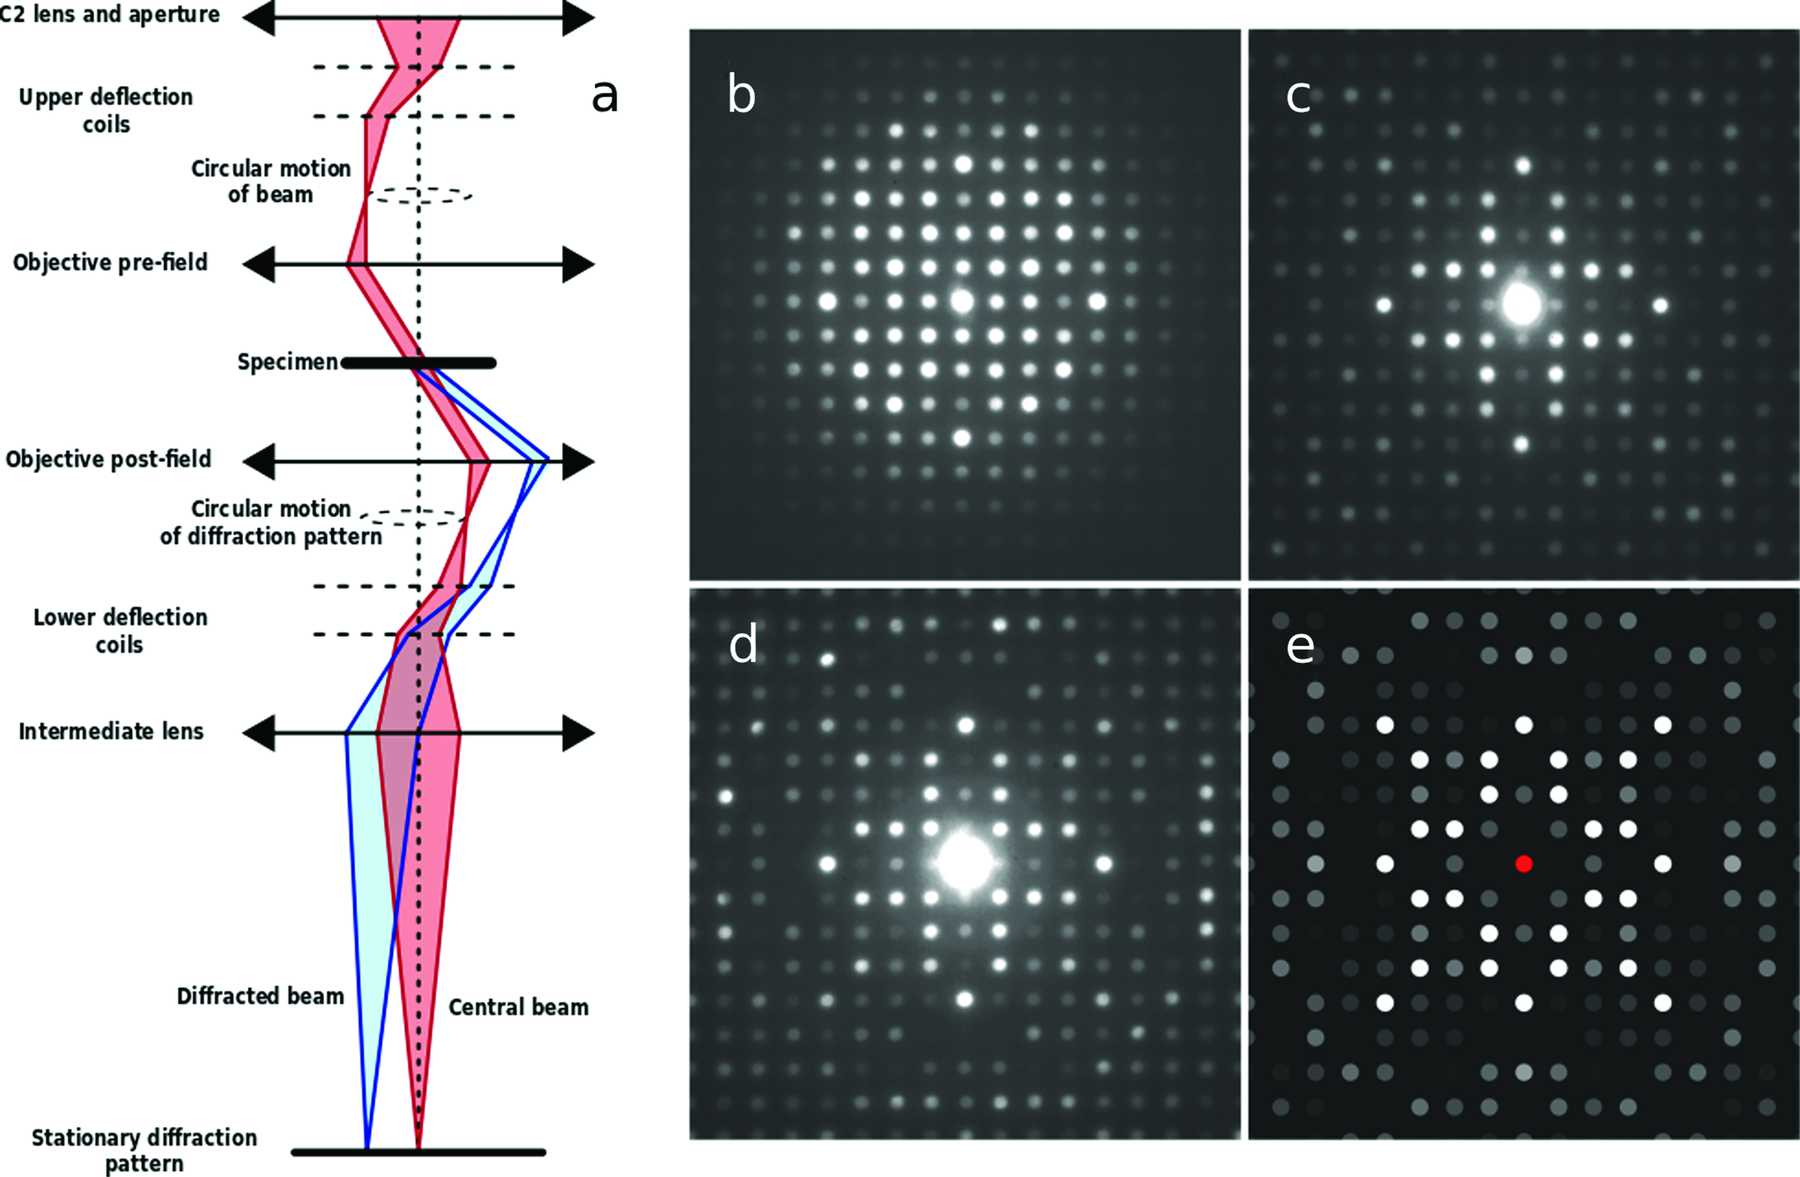
\includegraphics[width=0.7\linewidth]{fig/precession}
\caption{}
\label{fig:precession}
\end{figure}


\section{Data analysis}
	\subsection{(Introduction)}
	\subsection{Template matching}
Template matching is used for finding the location in a reference image where a template image fits best. The function \textit{MatchTemplate} in the python library OpenCV does this by sliding the template image over the reference image, and recording how well it fits at each point. This matching value is given as the normed square difference between the two images for each pixel in the reference image:
\begin{equation}
 R(x,y)= \frac{\sum_{x',y'} (T(x',y')-I(x+x',y+y'))^2}{\sqrt{\sum_{x',y'}T(x',y')^2 \cdot \sum_{x',y'} I(x+x',y+y')^2}}
 \label{eq:matching value}
\end{equation}

Here, $(x,y)$ are the coordinates of the reference image, $(x',y')$ the coordinates of the template, $I(x,y)$ is the value of the pixel $(x,y)$ in the reference image and $T$ likewise in the template. The matching value $R(x,y)$ can take any value between $0$ and $1$, where $0$ means a perfect match and $1$ a perfect mismatch.

	\subsection{Rescaling and rotating multidimensional data}
Attempting to rescale and rotate a multidimensional array can be problematic. A rotation that is not a multiple of 90 degrees will lead to jagged edges, and zero-values will have to be added to make it rectangular again. An even bigger problem is rescaling an array. If the new lengths along each axis are divisors of the original lengths, it is relatively easy. For example, rescaling a 10x10 array into a 5x5 array is simple as each value in the new array can be calculated as the mean of the corresponding 4 values (2x2) in the original array. This is called down-sampling, and causes information to be lost. Likewise, if rescaling the 10x10 into a 20x20 array, each value in the 10x10 array now corresponds to four values (2x2) in the 20x20 array. These four values can be given the same value as the one in the original array. This procedure is called up-sampling, and new information is added.
+++++ add figure to explain

However, if the new lengths of the array are not divisible by the original lengths, the rescaling procedure is no longer as easy to conceptualize. If instead of a two-dimensional array we now have a 3-dimensional one, where two of the dimensions are in real space and the third in signal space. This is the format of EDX data taken in STEM mode. Rescaling the real-space axes of this array will necessarily also change the signal axis. One way to solve this problem is to linearly interpolate the signal. The 10x10 array now denotes the real space of the EDX dataset. If it is down-sampled by a scale factor of $s=7.1$, it will become a 2x2 array. The top left value will now consist of the sum of the 7x7=49 top left values in the original matrix, plus 10 percent of the 8'th row and column. In the same way, the bottom right value will be the sum of the 2x2=4 bottom right values in the original matrix, plus 90 percent of the 8'th row and column. The array has now been linearly rebinned. 
